\chapter{Identasi}
\section{Penjelasan}
Identasi digunakan pada bahasa pemrograman python untuk menutup fungsi, spasi yang menjorok ke kanan digunakan untuk membedakan isi fungsi.
\par 
Jenis error yang akan ditemukan adalah IndentationError: unexpected indent, error yang saat identasi dari python tidak benar.
\begin{figure}[H]
    \centering
    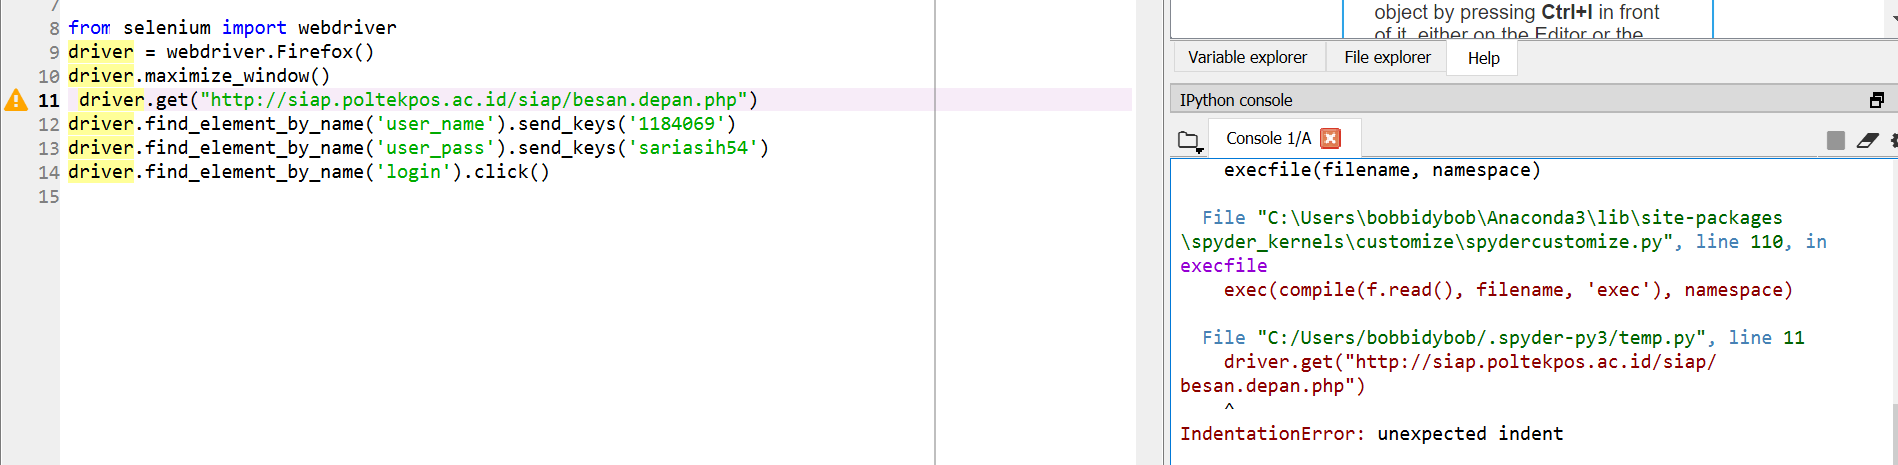
\includegraphics[scale=0.3]{figures/28.png}
    \label{28}
\end{figure}

Error akan terlihat di IPython console.

\par 
Cara menyelesaikan error tersebut dengan cara mengatur spasi sesuai kebutuhan, jika bagian code tersebut bukan merupakan fungsi maka tidak boleh diberi spasi sedangkan jika merupakan bagian dari isi fungsi, maka harus diberi spasi



Tutorial Selenium
\url{https://youtu.be/nF4MlIRyPOc}
